\documentclass[../main.tex]{subfiles}
\begin{document}
\setchapterstyle{kao}
\setchapterpreamble[u]{\margintoc}
\setchapterimage[6.5cm]{images/rubik-cubes.pdf}
\chapter[Groups: fundamental concepts]{Groups: fundamental concepts\footnotemark[0]}
\labch{groups-fund-conc}
%INIZIO LEZIONE 9
\section{Introduction}
The origin of the idea of group come from physics, as it happens for very many fundamental concepts of mathematics: it is a fundamental fact of nature that the transformations we can perform on a physical system in our laboratory (rotations, translations, Galilei transformations, Lorentz transformation) appear in "families" $\longrightarrow$ axiom of group. This "families" have remarkable properties. For example, we notice that if we apply two times the same transformation to our system, what we obtain is equivalent of applying one time a different transformation of the same kind (this is a property of a group).
\begin{marginfigure}[-2mm]
	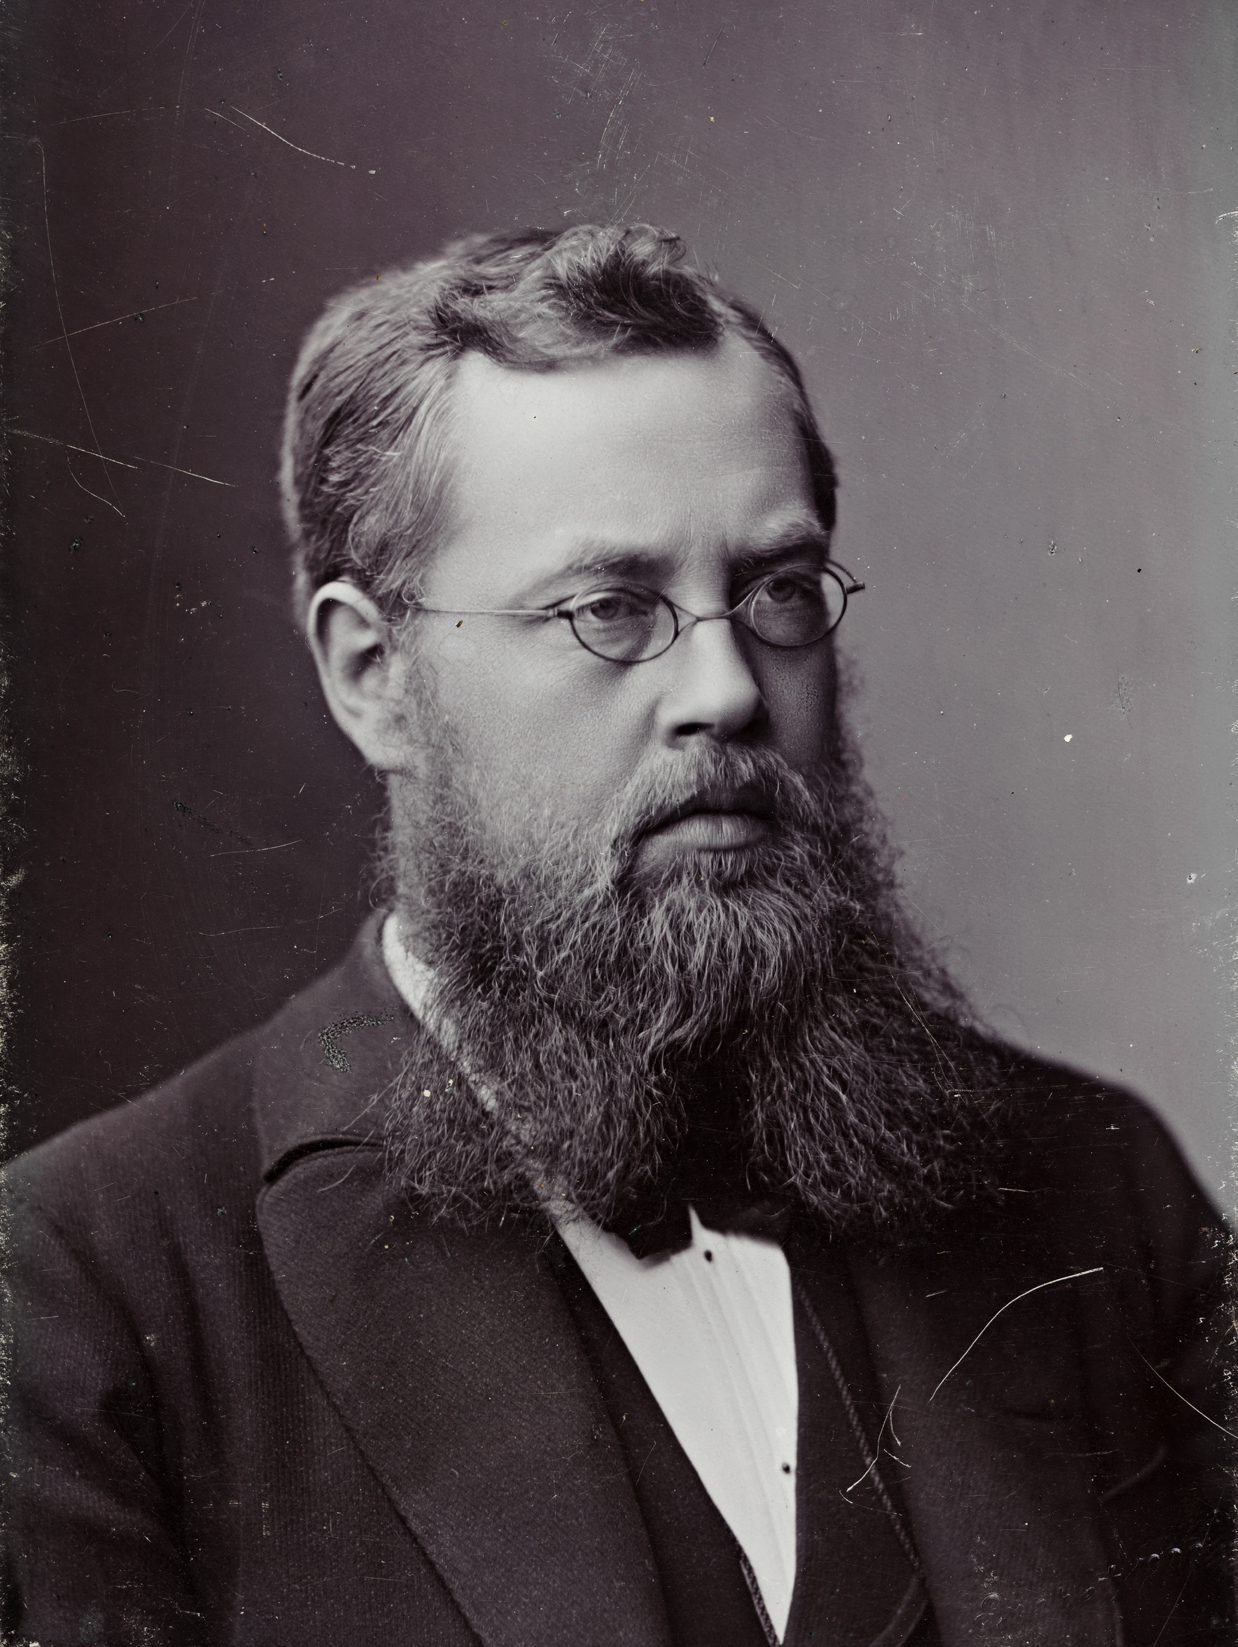
\includegraphics[width=1\linewidth]{images/Portrett_av_Sophus_Lie.jpg}
	\caption[Photo of Lie]{From \href{https://commons.wikimedia.org/wiki/File:Portrett_av_Sophus_Lie.jpg}{Wikimedia}: Portrait of Sophus Lie (1842-1899) of 1896 by the photographer: L. Szacinski (Christiania) Sted in Oslo Eier. Owner Institution: National Library of Norway. He died the in 1899 at the age of 56, due to pernicious anemia, a disease caused by impaired absorption of vitamin $\textrm{B}_{12}$.}
	\labfig{SophusLie}
\end{marginfigure}
At some point, a Norwegian mathematician, Sophus Lie (1842-1899, 57 y.o.) in \reffig{SophusLie}, understood that we can axiomatize this idea: from the concrete examples of groups of transformations (here group is used in the non-technical sense), we can define what nowadays is called group. Specifically, we can define what today is called a \textit{Lie group}, which are treated in \refch{Lie-groups-I}.
\newline
\newline
Notice that the life spawn of Sophus Lie has non-trivial intersection with the life of Lorentz, Poincarè, etc... (\reffig{Saphus-timeline}). He was scientifically active exactly at the time when people were computing the group of transformations which leaves invariant the Maxwell equations (\ref{eq:Maxwell-eq}), what is now called the \textit{Lorentz group}. He had the idea to axiomatize that, and it took many decades to reach the optimal set of axioms.\\
\begin{figure}[h!]
	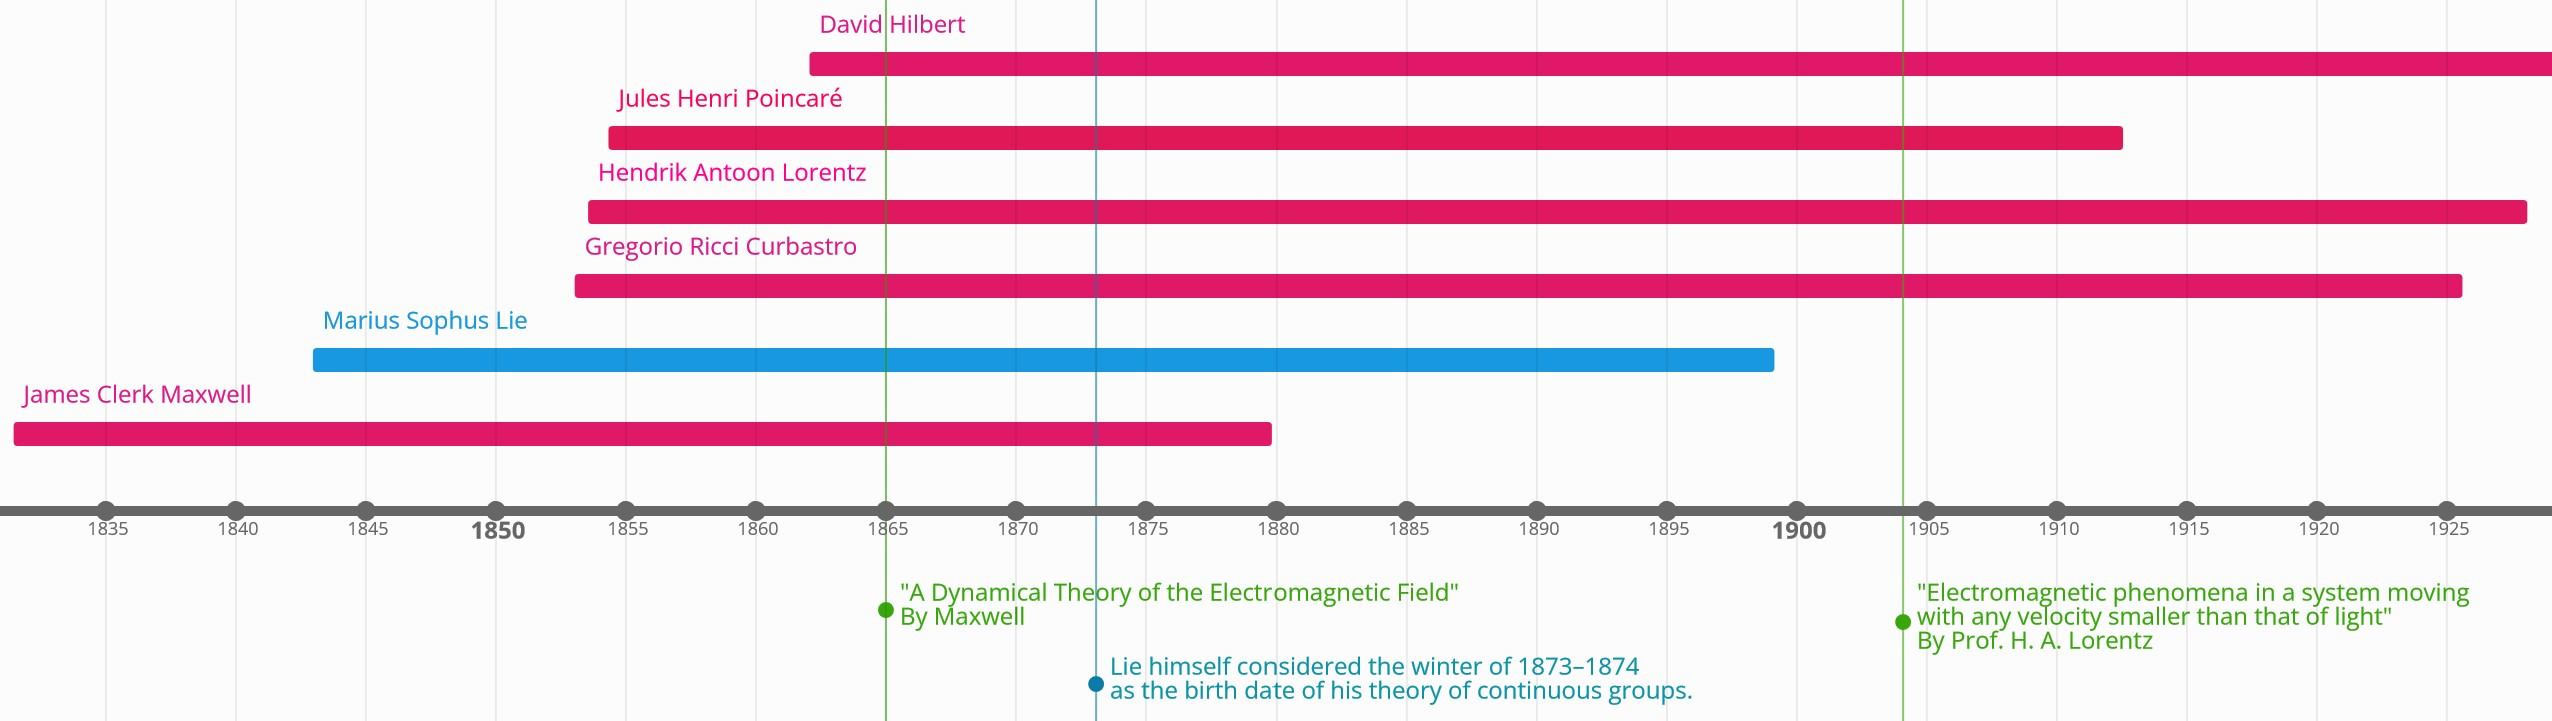
\includegraphics{images/Sophus_timeline.jpg}
	\caption{Timeline of Sophus life.}
	\labfig{Saphus-timeline}
\end{figure}
\section{Definitions}
\begin{definition}[Group - Gruppo]\index{Group}\labdef{group}
A \textbf{group} is a pair \(\pqty{G,\ast}\) where $G$ is a set and $\ast$ is a binary operation
\[
\begin{split}
\ast : G\times G& \to  G\\
(g,h) &\mapsto g\ast h
\end{split}
\]
satisfying the following properties: \renewcommand{\labelenumi}{(G\arabic{enumi})}
\begin{enumerate}
    \item Associativity: \( \forall \ g,h,l \in G\)
    \[
    \pqty{g\ast h}\ast l = g\ast \pqty{h\ast l}
    \]
    \item Neutral element\marginnote{It turns out that the neutral element is unique, but this is not in the axioms.}: \(\ \exists \ e \equiv e_\textrm{G}\) such that
    \[
    g\ast e = g = e \ast g \qquad \forall\ g\in G
    \]
    \item Inverse: \( \ \forall g\in G \ \ \exists \ g^{-1}\in G\) such that
    \[
    g^{-1}\ast g=e=g\ast g^{-1}
    \]
\end{enumerate}
\end{definition}
\begin{marginfigure}
	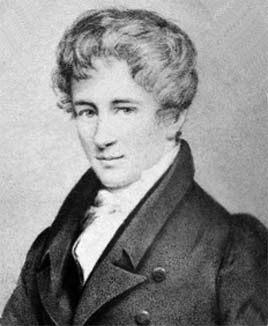
\includegraphics[width=1\linewidth]{images/Niels_Henrik_Abel.jpg}
	\caption[Photo of Niels Henrik Abel]{From \href{https://commons.wikimedia.org/wiki/File:Niels_Henrik_Abel.jpg}{Wikimedia}: Niels Henrik Abel (Norwegian: 5 August 1802 - 6 April 1829) was a Norwegian mathematician who made pioneering contributions in a variety of fields. He made his discoveries while living in poverty and died at the age of 26 from tuberculosis. The Abel Prize in mathematics, originally proposed in 1899 to complement the Nobel Prizes, is named in his honour.}
	\labfig{Abel}
\end{marginfigure}
There is a special, but relevant case: the \textit{Abelian groups}.
\begin{definition}[Abelian groups -  Gruppi abeliani]\index{Abelian groups}
A group is \textbf{abelian} if additionally holds true
\renewcommand{\labelenumi}{(G4)}
\begin{enumerate}
    \item Commutativity: \(\ \forall \ g,h\in G\)
    \[
    g\ast h = h\ast g
    \]
\end{enumerate}
\end{definition}
\begin{kaobox}[frametitle=Notation]
It is customary to write
\[
\begin{cases}
gh \ &\textrm{ for } \ g\ast h\\
g+h \ &\textrm{ for } \ g\ast h \ \textrm{ in the Abelian case}
\end{cases}
\]
\end{kaobox}
Now let us define another pair, which it is not very used since it lacks the inverse (or better, it is not always guaranteed for all the elements). 
\begin{definition}[Semigroup]
A \textbf{semigroup}\index{semigroup} is a pair \(\pqty{G,\ast}\) such that properties (G1) and (G2) are satisfied.
\end{definition}
Associativity is required in a semigroup, otherwise we get crazy with brackets.\marginnote{
\begin{kaobox}[frametitle=Notation]
We write $S \leq G$ ("$S$ is a subgroup of $G$).
\end{kaobox}
}
\begin{definition}[Subgroup - Sottogruppo]
A \textbf{subgroup} is a subset $S \subseteq G$ of a group $G$, such that
\[
\forall  g,h \in S \quad gh\in S \quad g^{-1}\in S
\]
\end{definition}
It is not true that every subset of a group is a subgroup, we have to check that if we take two elements in the subset, the product of them is still in the subset.
\begin{kaobox}[frametitle=Remark]
If $S\leq G$, then $(S,\ast \underset{\mathclap{\tikz \node {$\uparrow$} node [below=1ex]{\footnotesize $\big|_{S\times S}S\times S \to S$ };}}{\big|_{S\times S}})$ is a group.
\end{kaobox}
\section{Examples}
Let us now see some examples, organized in families.
\subsection{Groups of numbers}
These are examples that are already in our minds since the elementary school, simply we did not say they were groups.
\begin{example}
\((\mathbb{Z},+), \quad (\mathbb{Q}, +), \quad (\mathbb{R}, +), \quad (\mathbb{C}, +)\ \) are groups. They are subgroups of each other, in fact it holds \(\mathbb{Z}\leq \mathbb{Q}\leq\mathbb{R}\leq\mathbb{C}\), where the last relation is understood with respect to the addition\footnote{At the department of mathematics, some student could say that this is false: $\mathbb{R}$ can be embedded into $\mathbb{C}$, in fact $\mathbb{R}$ is isomorphic to a subgroup of $\mathbb{C}$. Chissene.}.\\
{\fontencoding{U}\fontfamily{futs}\selectfont\char 66\relax} $(\mathbb{N}, +)$ is not a group, it is a semigroup\marginnote[-5mm]{C'è un ultimo misterioso articolo di Richard Feynman a proposito. Prima di morire, scrisse un articolo in cui disse che la teoria quantistica fatta sugli spazi di hilbert complessi non è la teoria giusta, bensì la teoria giusta sarebbe quella che considera spazi di Hilbert su campi di caratteristica finita, ma grande
: $\mathbb{Z}^{\abs{p}}$, con $p$ numero primo molto molto grande, ma finito.}.
\end{example}
We can also consider the other operation, like
\begin{example}\labexample{grp-inv-elem}
Consider the \textbf{invertible elements} (with respect to multiplication) $\mathbb{A}^\times=\mathbb{A}\setminus\qty{0}$\marginnote{$\mathbb{A}$ stands for the set of algebraic numbers.}.\\ %For example, if $\mathbb{K}$ is the ??? number, this would be $\mathbb{K}^\times=\mathbb{K}\setminus\qty{0}$.\\
We can easily check that
\[
(\mathbb{Q}^\times, \cdot), \quad (\mathbb{R}^\times, \cdot), \quad (\mathbb{C}^\times, \cdot) \quad \textrm{are groups}
\]
{\fontencoding{U}\fontfamily{futs}\selectfont\char 66\relax} $(\mathbb{Z}^\times, \cdot)$ is not a group. We can restrict to unimodular numbers, for examples to complex numbers of modulus one U$(1)$ or to real numbers of modulus one (in this case there are just two elements\marginnote{In $\textrm{O}(1)$, $+1$ correspond to time reversal symmetry and $-1$ to (spatial) inversion symmetry.}):
\[
\begin{split}
\textrm{U}(1)&=\Bqty{z\in \mathbb{C}\  : \ \abs{z}=1}\\
\textrm{O}(1)&=\qty{x \in \mathbb{R}\  : \ \abs{x}=1}=\qty{+1,-1}
\end{split}
\]
$\qty(\textrm{U}(1),\cdot)$ and $\qty(\textrm{O}(1),\cdot)$ are groups with respect to multiplication. Again, all of these are related in the sense that some of them are subgroups of other, and they are nested in the obvious way:\marginnote{$\mathbb{C}^\times$ is the largest group (unless we want to consider also the quaternions $\mathbb{H}$).\\
This relation will be generalized to operators in \vrefexample{hilb-subgr-inver-unit-op}.}
\begin{equation}\labeq{unitary-group}
\begin{matrix}
\mathbb{Q}^\times &\leq & \mathbb{R}^\times &\leq &\mathbb{C}^\times\\
& {\rotatebox{-35}{$\geq$}} & {\rotatebox{90}{$\leq$}} & & {\rotatebox{90}{$\leq$}}\\
& & \textrm{O}(1) & \leq & \textrm{U}(1)\\
& & {\rotatebox{90}{$\leq$}}\\
& & \underset{\mathclap{\tikz \node {$\uparrow$} node [below=1ex]{\footnotesize smallest group };}}{\qty{1}}
\end{matrix}
\end{equation}
\end{example}
\subsection{Groups of functions}
\begin{example}
Let $\mathbb{K}$ be one of these numeric fields $\mathbb{K}\in\qty{\mathbb{Q},\mathbb{R},\mathbb{C}}$, let $\Omega$ be a set (any set, e.g. $\mathbb{R}^n$, a manifold, etc..), then we define a set of functions
\[
{\color{red}\pazocal{F}(\Omega,\mathbb{K})=\qty{f:\Omega \to \mathbb{K}}}\ni f,g
\]
we can equip it in a natural way, with a sum
\[
\big(f{\color{red}\underset{\mathclap{\tikz \node {$\uparrow$} node [below=1ex]{\footnotesize $\pazocal{F}(\Omega,\mathbb{K})$ };}}{+}}g\big)(\omega)=f(\omega)\underset{\mathclap{\tikz \node {$\uparrow$} node [below=1ex]{\footnotesize in $\mathbb{K}$ };}}{+}g(\omega)
\]
it can be checked that $\pqty{\pazocal{F}(\Omega, \mathbb{K}), {\color{red}+}}$ is an \textbf{Abelian group}.
\end{example}
We can play the same game with multiplications, we just have to remember that the function should take value in the set of invertible elements.
\begin{example}
Let $\mathbb{K}$ be one of these numeric fields $\mathbb{K}\in\qty{\mathbb{Q},\mathbb{R},\mathbb{C}}$, let $\Omega$ be a set (any set, e.g. $\mathbb{R}^n$, a manifold, etc..), then we define a set of functions
\[
{\color{red}\pazocal{F}(\Omega,\mathbb{K}^\times)=\qty{f:\Omega \to \mathbb{K}^\times}}\ni f,g
\]
we can equip it with
\begin{equation}\labeq{molt-betw-functs}
\big(f{\color{red}\underset{\mathclap{\tikz \node {$\uparrow$} node [below=1ex]{\footnotesize $\pazocal{F}(\Omega,\mathbb{K}^\times)$ };}}{\cdot}}g\big)(\omega)=f(\omega)\underset{\mathclap{\tikz \node {$\uparrow$} node [below=1ex]{\footnotesize in $\mathbb{K}^\times$ };}}{\cdot}g(\omega)
\end{equation}
it can be checked that $\pqty{\pazocal{F}(\Omega, \mathbb{K}^\times), {\color{red}\cdot}}$ is an \textbf{Abelian group}.
\end{example}
Actually, we can generalize this
\begin{example}(\textbf{New groups from old ones})\\
Let $\Omega$ be a set, and $G$ be a \textbf{group} (any), we can define
\[
{\color{red}\pazocal{F}(\Omega,G)=\qty{f:\Omega \to G}}\ni f,g
\]
since $G$ is a group, we can define the multiplications between functions, as we did for the multiplications between number in \refeq{molt-betw-functs}
\[
\big(f{\color{red}\underset{\mathclap{\tikz \node {$\uparrow$} node [below=1ex]{\footnotesize $\pazocal{F}(\Omega,G)$ };}}{\cdot}}g\big)(\omega)=f(\omega)\underset{\mathclap{\tikz \node {$\uparrow$} node [below=1ex]{\footnotesize in $G$ };}}{\cdot}g(\omega)
\]
\paragraph{\underline{Exer:}} Check that $\pazocal{F}(\Omega,G)$ is a group (Abelian if $G$ is Abelian).
\paragraph{\underline{Subex:}} Consider $\Omega=\mathbf{M}$ manifold on $G=\textrm{U}(1)$. Then
\[
{\pazocal{F}(\Omega,\textrm{U}(1))=\qty{f:\Omega \to \textrm{U}(1)}}\ni f,g
\]
which we can also write $f(x)=e^{ig(x)}$. We recognize an object that is familiar in physics:
\[
{\pazocal{F}^\infty(\mathbf{M},\textrm{U}(1))=\qty{f:\mathbf{M} \xrightarrow{C^\infty} \textrm{U}(1)}}
\]
Therefore the set of all \textbf{(smooth) gauge transformations} ($A'=A\pm \nabla g$) is an \textbf{Abelian group}. 
\end{example}
\subsection[Group of endomorphisms/matrices/operators]{Group of endomorphisms/matrices/operators\sidenote{We put all together, because each example generalize the previous. Another problem is that each lecturer of geometry will use a different terminology.}}
\todo{Hereafter, fix $\mathbb{K}\in\Bqty{\mathbb{Q},\mathbb{R},\mathbb{C}}$}
The examples we saw are interesting, but not so interesting to justify the use of the group theory. The theory becomes non trivial and interesting when the group is not Abelian anymore. For physicist these are %groups of ??? or
groups of operators, which naturally appear in quantum mechanics.\marginnote[5mm]{From Chapter 5 and 7 of \cite{abate2006geometria}:\\
\textbf{Definizione.} \ Un'\textit{applicazione} (o \textit{trasformazione}) \textit{lineare} fra due spazi vettoriali $V$ e $W$ definiti su un campo $\mathbb{K}$, è una funzione $T:V\to W$ tale che:
\begin{enumerate}
    \item $T(v_1+v_2)=T(v_1)+T(v_2)$  $\forall \ v_1, v_2\in V$ (diremo che $T$ è \textit{additiva});
    \item $T(\lambda v)=\lambda T(v)$ per tutti i $\lambda\in\mathbb{K}$ e $v\in\ V$ (diremo che T è \textit{omogenea}).
\end{enumerate}
In altre parole, un'applicazione lineare trasforma (rispetta, conserva) le operazioni dallo spazio di partenza a quello d'arrivo. Se $V=W$, si parla di \textit{endomorfismo} (od \textit{operatore lineare}).\\
\textbf{Definizione:} Diremo che un'applicazione lineare $T:V\to W$ è \textit{invertibile} se esiste un'applicazione \textit{lineare} $S:W\to V$, l'\textit{inversa} di $T$, tale che $T\circ S = \textrm{id}_W$ e $S \circ T = \textrm{id}_V$. L'inversa, se esiste, si indica con $T^{-1}$.\\
\textbf{Proposizione:} Sia $T:V\to W$ un'applicazione lineare. Allora $T$ è invertibile se e solo se è inettiva e surgettiva.\\
\textit{Dimostrazione.} Se $T$ è invertibile è chiaramente bigettiva. Viceversa, supponiamo $T$ iniettiva e surgettiva; allora esiste la funzione inversa $S:W\to V$. Dobbiamo solo dimostrare che $S$ è lineare. Prendiamo $w_1$ e $w_2\in W$; essendo $T$ surgettiva, esistono $v_1,v_2\in V$ tali che si abbia $T(v_1)=w_1$ e $T(v_2)=w_2$. Allora $T(v_1+v_2)=w_1+w_2$; applicando $S$ otteniamo $S(w_1+w_2)=v_!+v_2=S(w_1)+S(w_2)$. Analogamente si dimostra che $S(\lambda w_1)=\lambda S(w_1)$.
}
\begin{definition}[Endomorphism or linear operator]\index{Endomorphism}\index{Linear operator}
Let $\textrm{V}$ be a vector space over the field $\mathbb{K}$, then an endomorphism is defined as all the maps such that
\[
\textrm{End}(\textrm{V})=\Bqty{A:V\xrightarrow[\textrm{linear}]{}V}
\]
\end{definition}
With these maps we can do sums and compositions.
\begin{example}\labexample{general-linear-group}
For $A,B\in \textrm{End}(V)$ then
\[
\begin{split}
\pqty{A+B}v&=Av+Bv \quad  \quad \forall \ v\in V\\
\pqty{A\circ B}v&=A\pqty{Bv}\quad  \qquad \forall \ v\in V
\end{split}
\]
It can be checked that $\pqty{\textrm{End}(V),+}$ is an \textbf{Abelian group}.\\
How about with respect to multiplication? In that case, it is not a group, because there a lot of not invertible elements. We should consider the so called \textbf{General Linear group}\index{General linear group}, which is the group of all invertible elements of $\textrm{End}(V)$, i.e.
\begin{equation}\labeq{General-Linear-group}
\textrm{GL}(V)=\Bqty{A: V\xrightarrow[\textrm{linear}]{}V \ \textrm{s.t. $A$ is invertibile}}
\end{equation}
The inverse $A^{-1}$ is automatically linear and invertibile, so is in $\textrm{GL}(V)$. $\pqty{\textrm{GL}(V),\circ}$ is a \textbf{group}.
\end{example}
If we require that $\textrm{dim}(V)<+\infty$, then there is a correspondence between endomorphisms and matrices
\[
\begin{split}
\psi_e : \textrm{End}(V)& \to  \textrm{Mat}(n,\mathbb{K})\\
A &\mapsto \pqty{A^i_{\;\;j}}
\end{split}
\]
where the endomorphism is given by a linear basis\sidenote{With $e$ we are not indicating here the neutral element.} $\underline{e}=\pqty{e_1,\dots,e_n}$ and $ \pqty{A^i_{\;\;j}}$ is defined by
\[
Ae_j=\sum_{l=1}^n A^l_{\;\;j}e_l \qquad \Big|\Big| \quad \star
\]
This identifies endomorphisms with matrices, whenever the spaces are finite dimensional. Notice that the Ricci's calculus is useful also in this elementary problem.\marginnote[-25mm]{We write the matrix with indices at different levels, because then when we have to expand in the linear combination of the bases, everything goes in the right place.}
\[
\begin{split}
    \pqty{A+B}^i_{\; \; j}&=A^i_{\;\;j}+B^i_{\;\;j}\\
    \pqty{AB}^i_{\;\;j}&=\sum_{l=1}^n A^i_{\;\;j}B^i_{\;\;j}
\end{split}
\qquad A^{\overset{\mathclap{\tikz \node {$\downarrow$} node [above=1.25ex] {\footnotesize row};}}{i}}_{\;\;\underset{\mathclap{\tikz \node {$\uparrow$} node [below=1.25ex] {\footnotesize column };}}{j}}
\]
If we have a basis, we can then identify the general linear group defined in \refeq{General-Linear-group} as the set of endomorphism with determinant different from zero
\[
\textrm{GL}(V)=\Bqty{A\in \textrm{End}(V): \ \textrm{det}(A)\neq 0}
\]
The fact that the space is finite dimensional plays a very minor role.
\begin{marginfigure}[-20mm]
     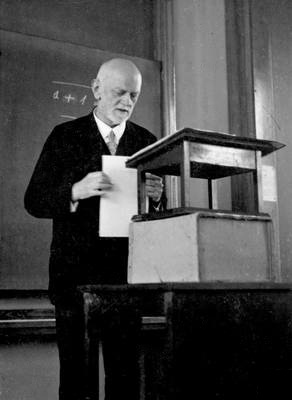
\includegraphics[width=1\linewidth]{images/David_Hilbert_Vorlesung_1932.jpg}
     \caption[Photo of Hibert]{From \href{https://commons.wikimedia.org/wiki/File:David_Hilbert_Vorlesung_1932.jpg?uselang=it}{Wikimedia}: The mathematician David Hilbert in a lecture 1932.}
 \end{marginfigure}
\begin{marginfigure}
	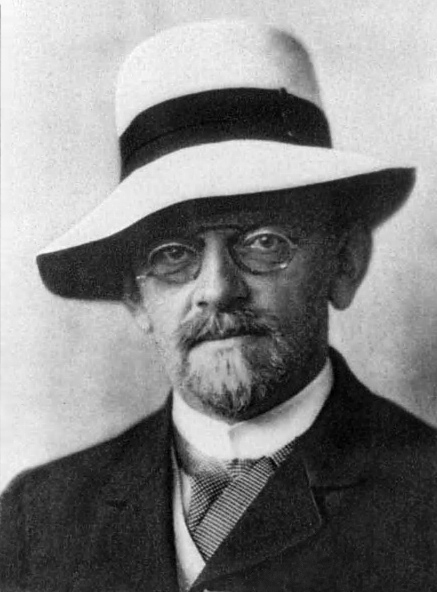
\includegraphics[width=1\linewidth]{images/Hilbert.jpg}
	\caption[Photo of Hibert]{From \href{https://commons.wikimedia.org/wiki/File:Hilbert.jpg}{Wikimedia}: David Hilbert (23 January 1862 – 14 February 1943), wearing a dashing hat in 1912. He was a German mathematician born in Königsberg, East Prussia (now Kaliningrad, Russia) who is recognized as one of the most influential mathematicians of the XIX and early XX centuries.}
	\labfig{Hilbert}
\end{marginfigure}
\begin{example}
Let $\mathcal{H}$ be a complex Hilbert space (in general it will be infinite dimensional), we could play the same game as before, but if we consider all the linear transformation of this space, we get a huge and unpractical set. So, what is useful, is to restrict to those linear transformation which are also continuous. Therefore, the relevant object (the analogous of the endomorphism) will be
\[
\begin{split}
\pazocal{B}(\mathcal{H})=\big\{A:\mathcal{H}&\xrightarrow[\underset{\mathclap{\tikz \node {$\big\updownarrow$} node [below=1.25ex] {\footnotesize Bounded };}}{\text{\parbox{1.3 cm}{\centering linear \\[-4pt]  continuous}}}]{}\mathcal{H}\big\}\\[-2.5mm]
\norm{A}:=\sup_{\psi\neq 0}\frac{\norm{A\psi}}{\norm{\psi}}=\sup_{\norm{\psi}=1}&\norm{A\psi}\overset{\mathclap{\tikz \node {$\big\downarrow$} node [above=0ex] {\footnotesize};}}{<}+\infty
\end{split}
\]
To be smaller than infinity is the definition of bounded (\textit{limitato) }for a linear operator\index{Bounded operator}, and it is equivalent to be continuos. So what is useful is to take the set of all linear bounded operators, which is still infinite dimensional, but more tractable than the huge set of all the possible linear operators. We can equip it with operations:\\
For $A,B\in \pazocal{B}(\mathcal{H})$ then
\[
\begin{split}
\pqty{A+B}\psi&=A\psi+B\psi \quad  \quad \forall \ \psi\in \mathcal{H}\\
\pqty{A\circ B}\psi&=A\pqty{B\psi}\qquad  \,\quad \forall \ \psi\in \mathcal{H}
\end{split}
\]
$\pqty{\pazocal{B}(\mathcal{H}),+}$ is an \textbf{Abelian group}.
\end{example}
\begin{example}\labexample{hilb-subgr-inver-unit-op}
If want to have something with a product, we should not take all $\pazocal{B}(\mathcal{H})$, because there are a lot of non-invertibile elements, but to take something which is written like the following and that identifies only the continuos invertible elements:
\[
\begin{split}
\pazocal{B}(\mathcal{H})^\times &= \Bqty{A\in\pazocal{B}(\mathcal{H}): A \ \textrm{is invertibile with} \ A^{-1}\in\pazocal{B}(\mathcal{H})}\\
&\neq \pazocal{B}(\mathcal{H}) \setminus \Bqty{0}
\end{split}
\]
$\pqty{\pazocal{B}(\mathcal{H})^\times,\circ}$ is a \textbf{group}. (NON ABELIAN!)
\end{example}
\begin{example}\labexample{unitary-op}
Since the Hilbert space is an additional structure\marginnote{The additional structure is the hermitian (or inner) product.}, with respect to the linear structure, then we can define a subgroup as the group of all the unitary operators:
\[
\pazocal{U}(\mathcal{H})=\Bqty{U\in\pazocal{B}(\mathcal{H}): \ UU^\ast = \mathbb{1}=U^\ast U}
\]
It can be checked that $\pqty{\pazocal{U}(\mathcal{H}), \circ}$ is a \textbf{group} and $\underline{\pazocal{U}(\mathcal{H})\leq\pazocal{B}(\mathcal{H})^\times}$.\footnote{It is easy to check because the composition of two unitary operation is still unitary and the inverse of a unitary operator is the adjoint of the operator, which is still unitary.} This relation is the generalization of the relation (\ref{eq:unitary-group}) in \vrefexample{grp-inv-elem}, where $\pazocal{B}(\mathcal{H})^\times$ plays the role of $\mathbb{C}^\times$ and $U(1)$ is replaced by the group of all the unitary operators, instead of having just the group of unimodular numbers.
\end{example}
All the examples we made, would have they worked with another space? For example if, instead of considering a complex Hilbert space, we would have considered a \href{https://it.wikipedia.org/wiki/Spazio_di_Banach}{Banach space}\sidenote{In mathematics, more specifically in functional analysis, a Banach space is a complete normed vector space. Thus, a Banach space is a vector space with a metric that allows the computation of vector length and distance between vectors and is complete in the sense that a Cauchy sequence of vectors always converges to a well defined limit that is within the space.}. Then the notion of bounded operator still exists (and it is still the same), it is still good because every linear bounded operator is also continuous and we can still define operation in the same way. The need to consider an Hilbert space arises when we talk about the \textit{unitary operators} (\refexample{unitary-op}): if we have an Hilbert space, the Hermitian product on the Hilbert space induces the notion of \textit{adjoint} of an operator (which otherwise does not exist, this is based on the inner product). Once we have the adjoint we can define two things:
\begin{enumerate}
    \item \textbf{Self adjoint operators}, which are the analogous of real numbers
    \item \textbf{Unitary operators}, which are the analogous of unimodular numbers
\end{enumerate}
So we have this relevant subgroup of unitary operators, which otherwise, in a general Banach space, is not there. In the Banach case, we can still define the subgroup of operators which preserve the Banach norm (a norm such that $\forall x, y \in A, \|x \, y\| \ \leq  \|x \| \, \| y\|$): this is the group of \textit{isometries}\index{Group of isometries}, but it not the same and it is not so nice. \sidenote{If $X$ and $Y$> are normed spaces over the same ground field $\mathbb{K},$ the set of all continuous $\mathbb{K}$-linear maps $T : X \to Y$ is denoted by $B(X, Y).$ In infinite-dimensional spaces, not all linear maps are continuous. A linear mapping from a normed space $X$ to another normed space is continuous if and only if it is bounded on the closed unit ball of $X$. Thus, the vector space $B(X, Y)$ can be given the operator norm
\[\|T\| = \sup \left\{\|Tx\|_Y \mid x\in X,\ \|x\|_X \leq 1 \right\}\]
For $Y$ a Banach space, the space $B(X, Y)$ is a Banach space with respect to this norm.
If $X$ is a Banach space, the space $B(X) = B(X, X)$ forms a unitary Banach algebra; the multiplication operation is given by the composition of linear maps.\\
If $X$ and $Y$ are normed spaces, they are \textbf{isomorphic normed spaces} if there exists a linear bijection $T : X \to Y$ such that $T$ and its inverse $T^{-1}$ are continuous. If one of the two spaces $X$ or $Y$ is complete (or reflexive, separable, etc.) then so is the other space. Two normed spaces $X$ and $Y$ are \textbf{isometrically isomorphic} if in addition, $T$ is an isometry, that is, $\|T(x)\| = \|x\|$ for every $x$ in $X$.} %min 23 L10
There is a global exercise we propose.\\
\begin{exercise}
Check that \textbf{some} of the examples before are indeed groups (or Abelian groups when is the case), i.e. they satisfy (G1), (G2) and (G3).
\end{exercise}
\subsection[Other examples]{Other examples - Fix $\mathbb{K}\in\Bqty{\mathbb{Q},\mathbb{R},\mathbb{C}}$}
\begin{marginfigure}[35mm]
	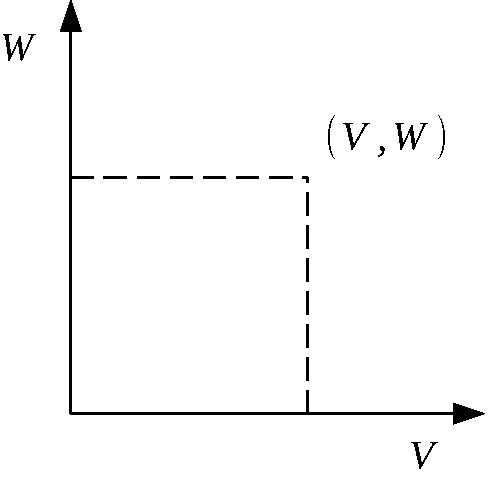
\includegraphics[width=1\linewidth]{images/linear_space_group.pdf}
	\caption{$V\oplus W$ as Cartesian product.}
	\labfig{lin-sp-group}
\end{marginfigure}
\begin{example}
Let $\pazocal{V}_{\textrm{ect}}$ be the set of all the possible finite dimensional linear spaces
\[
\pazocal{V}_{\textrm{ect}}=\Bqty{\textrm{Linear space over $\mathbb{K}$ with} \ \textrm{dim}V<+\infty}
\]
Let $V,W\in\pazocal{V}_{\textrm{ect}}$. We define $V\bigoplus W$ as a vector space (which is a triple), in which the set is just the Cartesian product and we define the two binary operations component-wise
\[
\begin{split}
    \textrm{Set:} \quad & V\oplus W = V \times W = \Bqty{(v,w): \ v\in V, \ w\in W}\\
    \textrm{I operat. :} \quad & (v_1,w_1) {\color{red}+}(v_2,w_2)=(v_1+v_2,w_1+w_2)\\
    \textrm{II operat. :} \quad &\lambda{\color{red}\cdot}(v,w)=(\lambda w,\lambda v)
\end{split}
\]
So $\forall \ V,W\in\pazocal{V}_{\textrm{ect}}$ we define $V\oplus W\in\pazocal{V}_{\textrm{ect}}$. We took two vector spaces, did the direct product and the result is still a vector space. Then we define a binary operation from the set of all the possible vector spaces to the set of all the possible vector spaces to itself:
\[
\begin{split}
\oplus : \pazocal{V}_{\textrm{ect}}\times \pazocal{V}_{\textrm{ect}}& \to  \pazocal{V}_{\textrm{ect}}\\
(V,W) &\mapsto V\oplus W
\end{split}
\]
\underline{Question 1:} Is the pair $\pqty{\pazocal{V}_{\textrm{ect}}, \oplus}$ a group?? Since the direct sum is associative, there is a neutral element such that, replacing equalities with isomorphisms,
\[
\begin{split}
    V \oplus E &\to V\\
    (v,0) &\mapsto v
\end{split}\quad
\textrm{with } \ E=\Bqty{0}
\]
We understand that we do not have to take the set of vector spaces, but the set of vector spaces \textit{up} to a isomorphism, so the refined question is\\
\underline{Question 2:} $\pqty{\pazocal{V}_{\textrm{ect}}\big/\cong, \oplus}$ is a group? No, it is not a group, because there a no inverse, but it is a \textbf{semigroup}.
\end{example}
\begin{marginfigure}[-80mm]
    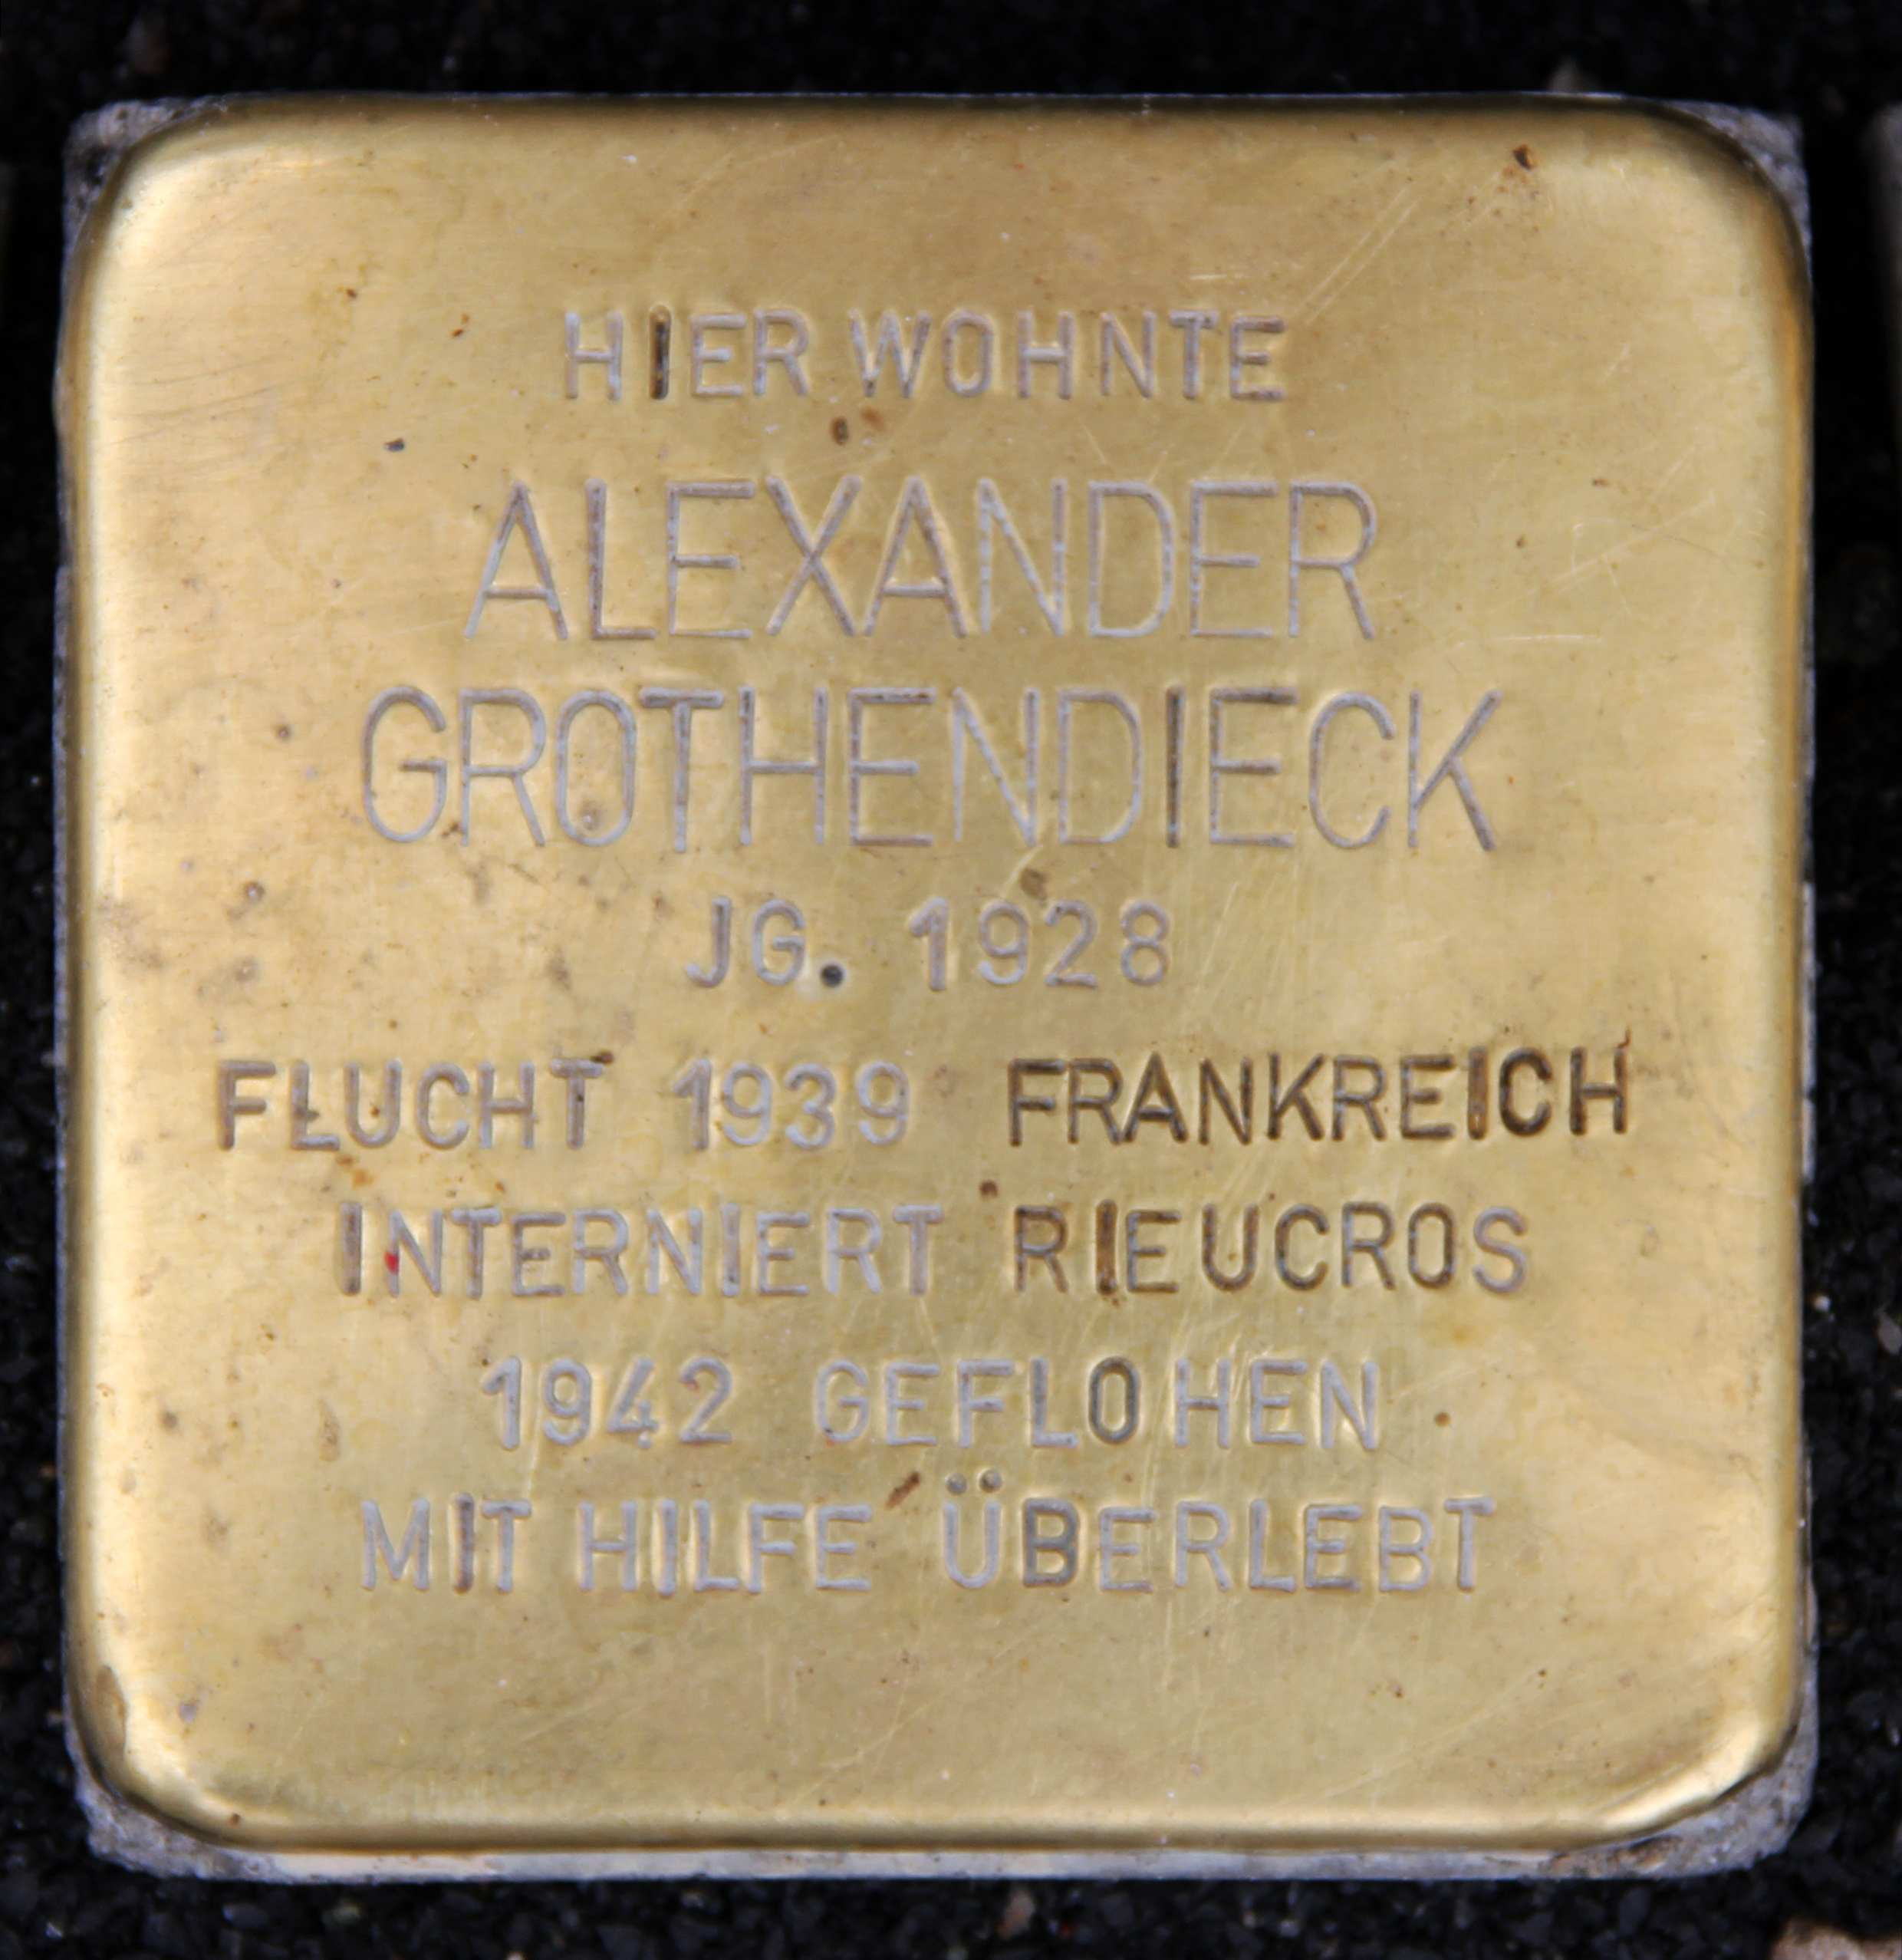
\includegraphics[width=1\linewidth]{images/Stolperstein_Brunnenstr_165_(Mitte)_Alexander_Grothendieck.jpg}
    \caption[stumbling block of Alexander Grothendieck]{From \href{https://commons.wikimedia.org/wiki/File:Stolperstein_Brunnenstr_165_(Mitte)_Alexander_Grothendieck.jpg}{Wikimedia} "Stolperstein" (stumbling block - \textit{pietra d'inciampo}), Alexander Grothendieck, Brunnenstraße 165, Berlin-Mitte, Germany.}
\end{marginfigure}
\begin{marginfigure}[-10mm]
	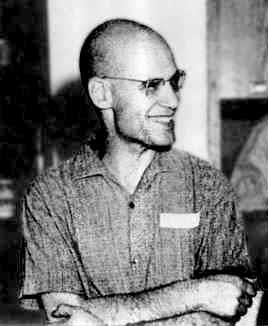
\includegraphics[width=1\linewidth]{images/Alexander_Grothendieck.jpg}
	\caption[Photo of Alexander Grothendieck]{From \href{https://commons.wikimedia.org/wiki/File:Alexander_Grothendieck.jpg}{Wikimedia}: Alexander (or Alexander) Grothendieck (28 March 1928 – 13 November 2014) in Montreal, 1970. He was a stateless (\textit{apolide}) and then French mathematician who became the leading figure in the creation of modern algebraic geometry. In 1991, he moved to the French village of Lasserre in the Pyrenees, where he lived in seclusion, still working tirelessly on mathematics and his philosophical and religious thoughts until his death in 2014.}
	\labfig{Grothendieck}
\end{marginfigure}
However, there is a standard trick to pass from semigroups to groups and it is essentially the one learned in elementary school\sidenote{At the beginning there were just natural numbers, then at some point appear the negative numbers. We can look at the as derived ?? objects, i.e. space of natural number in which the difference is constant, so to speak.}: the same construction which brings from $\pqty{\mathbb{N},+}$ to $\pqty{\mathbb{Z},+}$ yield a "completion" of $\pqty{\pazocal{V}_{\textrm{ect}}\big/\cong, \oplus}$, which is called the \textbf{\href{https://it.wikipedia.org/wiki/Gruppo_di_Grothendieck}{Grothendieck group}}.\index{Grothendieck group}
It is a group whose elements are isomorphic to theirself ?? of vector spaces and in which the sum is a direct sum, the neutral element is the zero dimensional vector space and, in a sense, he invented an inverse (which should have a negative dimension, but it is not a true vector space) in such a way that the direct sum of a vector space with ?? ?? ?? is isomorphic to the trivial one.
\subsection{New groups from old ones}
\begin{example}
Let $G_1$ and $G_2$ be groups (each one with its operation). We want to define the direct product of groups, namely a new group\footnote{Even if it is the same symbol, we are not referring to the tensor product here with $\otimes$.} $G_1\otimes G_2$ (or also $G_1 \odot G_2$ to avoid confusion). This direct product of group is, remembering that a group is a pair with a set (the Cartesian product in our case) and an operation that we need to define
\[
\begin{split}
    G \otimes H &= \pqty{G\overset{\textrm{set}}{\times} H,\ {\color{red}\cdot}}\\
    (g_1,h_1){\color{red}\cdot}(g_2,h_2)&=(g_1g_2,h_1h_2)
\end{split}
\]
\end{example}
\begin{exercise}
Check that $G\otimes H$ is a group (satisfies (G1), (G2) and (G3) of \vrefdef{group}). If both $G$ and $H$ are Abelian, also the direct product is Abelian.
\end{exercise}
\section[Homomorphisms]{Homomorphisms (of groups)}
Now we need to say when two groups should be identified with the same object, as we did with linear spaces.
\begin{definition}[Homomorphism]
Let $\overset{(G,\ast_G)}{G}$ and $\overset{(H,\ast_H)}{H}$ be groups. An \textbf{homomorphism (of groups)} [shortly: \textbf{morphism}]\index{homomorphism (of gorups)}\index{morphism} is a map
\[
\varphi: G \to H
\]
which "preserves the product" i.e.
\marginnote{\begin{kaobox}[frametitle=Terminology]
\[\underset{\mathclap{\tikz \node {$\downarrow$} node [below=0.4ex]{\footnotesize \parbox{1.3 cm}{\centering "The same \\[-4pt]  operations"}};}}{\textrm{homo}}\neq\overset{\mathclap{\tikz \node {$\uparrow$} node [above=0.4ex]{\footnotesize Open sets};}}{\textrm{homeo}}\textrm{-morphism}\]
We will mainly use the first one.
\end{kaobox}}
\[
\begin{split}
    \varphi(gh)&=\varphi(g)\varphi(h) \qquad \forall \ g,h \in G\\
    \text{\parbox{1.3 cm}{\centering Pedantic \\[-4pt] notation}} \quad \varphi(g\ast_G h)&=\varphi(g)\ast_H \varphi(h)
\end{split}
\]
\end{definition}
\begin{kaobox}[frametitle=Notation]
The set of all the homomorphisms from $G$ to $H$ is denoted by $\textrm{Hom}(G,H)$
\end{kaobox}
\begin{definition}[Kernel - nucleo]
The kernel\footnote{Viene spesso indicato come $\ker ( f )$, dal tedesco \textit{Kern}. In linear algebra is the set of elements whose image is zero.} of a homomorphism $\varphi: G\to H $ is the set of elements whose image is the neutral element:
\[
\begin{split}
\ker\varphi&=\Bqty{g\in G: \varphi(g) = e_H}\\
\Im\varphi&=\Bqty{h\in H: \exists \ g\in G \big| \ h=\varphi(g)}
\end{split}
\]
\end{definition}
Let us see some examples
\begin{example}
If we consider
\[
\begin{split}
    \pqty{\mathbb{R},+}&\to \pqty{\mathbb{C}^\times,\cdot}\\
    x \ &\mapsto\ e^{ix}
\end{split}
\]
We notice that
\[
\begin{split}
\ker(\varphi)&=\Bqty{x\in \mathbb{R}: e^{ix} = 1}\;=2\pi\overset{\text{\parbox{0.4 cm}{\centering $(\mathbb{R},+)$ \\[-4pt]  {\rotatebox{90}{$\leq$}}}}}{\mathbb{Z}}\textrm{ is a group}\\
\Im(\varphi)&=\Bqty{z\in \mathbb{C}^\times: z=e^{ix}}=\underset{\text{\parbox{0.6 cm}{\centering  {\rotatebox{90}{$\geq$}}\\[-4pt] $\mathbb{C}^\times$ }}}{\textrm{U}(1)}\textrm{ is a group}
\end{split}
\]
\end{example}
The example above is interesting: we have a morphism of group of numbers, and we see that the kernel of the morphism is a subgroup of the source and the image is a subgroup of the target group. This is a very general fact, that we prove further on in the \refthm{ker-im-subgroup}. The example above has a very natural and useful generalization to operators
\begin{example}
Let us take the set of bounded self-adjointed operators over a (separable, complex) Hilbert:
\[
\pazocal{B}_{\textrm{sa}}(\mathcal{H})=\Bqty{A\in\pazocal{B}(\mathcal{H}):A^\ast=A}
\]
\begin{exercise}
Check that $\pqty{\pazocal{B}_{\textrm{sa}}, +}$ and $\pqty{\pazocal{U}_{\textrm{sa}}, \circ}$ are groups.
\end{exercise}
\end{example}
As we can already imagine, what is written above for numbers, generalise to operators: real numbers are replaced by self adjointed operators
\[
\begin{split}
\varphi = \pazocal{B}_{\textrm{sa}}(\mathcal{H}) &\to \pazocal{U}(\mathcal{H})\\
A&\mapsto e^{iA}:=\sum_{n=0}^\infty \frac{1}{n!}A^n\marginnote{The series is convergent because the operator is bounded, we will come back to it later.}
\end{split}
\]
It is not obvious who are the kernel and the image, but still the general \refthm{ker-im-subgroup} tells us that the kernel is a subgroup of the addictive group of self adjointed bounded operators and the image, that is inside the group of unitary operator, is also a group.
\begin{proposition}\labprop{neutral-el-hom}
Let $G$ and $H$ be groups and $\varphi\in\textrm{Hom}(G,H)$. Then
\begin{enumerate}
    \item \begin{equation}\labeq{neutral-el-hom-I}
        \varphi(e_G)=e_H
    \end{equation}
    \item \begin{equation}\labeq{neutral-el-hom-II}
        \varphi(g^{-1})=\varphi(g)^{-1}
    \end{equation}
\end{enumerate}
\end{proposition}
\begin{proof} \textbf{1.}
\[
\varphi(g)\cdot e_H = \varphi (g) =\varphi\pqty{g e_G} \overset{\mathclap{\tikz \node {$\downarrow$} node [above=1.25ex] {\footnotesize $\varphi\in\textrm{Hom}(G,H)$};}}{=}\varphi(g)\underset{\mathclap{\tikz \node {$\uparrow$} node [below=1ex]{\footnotesize in $H$ };}}{\cdot}\varphi(e_G)
\]
Multiply by $\varphi(g)^{-1}$ [$\exists$ by (G3)]\sidenote{(G3): $g^{-1}\ast g=e=g\ast g^{-1}$} on the left:
\[
\begin{WithArrows}\WithArrowsOptions{displaystyle}
\varphi(g)^{-1}\big(\varphi(g)\cdot e_H\big)&=\varphi(g)^{-1}\big(\varphi(g)\varphi(e_G)\big)\Arrow{(G1):\\the product is associative}\\
\underbrace{\left(\varphi(g)^{-1}\varphi(g)\right)}_{\color{red}=e_H}\cdot e_H&=\underbrace{\left(\varphi(g)^{-1}\varphi(g)\right)}_{\color{red}=e_H}\varphi(e_G)\Arrow{By definition\\of the inverse}\\
e_H=e_H\cdot e_H &= e_H\cdot \varphi(e_G)=\varphi(e_G)
\end{WithArrows}
\]
Then $e_H=\varphi(e_G)$\marginnote{This was very formal just to emphasize the role of axioms. It will be quicker in the following pages.}
\end{proof}
\begin{proof}\textbf{2.}
\[
\begin{WithArrows}\WithArrowsOptions{displaystyle}
\varphi(e_G)&=\varphi(g^{-1}g) \Arrow{$\varphi\in\textrm{Hom}(G,H)$}\\
\varphi(e_G)&=\varphi(g^{-1})\varphi(g)\Arrow{{\color{blue}$\times\varphi(g)^{-1}$} to the r.h.s.}\\
\boxed{\varphi(g)^{-1}}=e_H\cdot\varphi(g)^{-1}\overset{(\ref{eq:neutral-el-hom-I})}{=}\varphi(e_G)\cdot{\color{blue}\varphi(g)^{-1}}&=\Big(\varphi(g^{-1})\varphi(g)\Big){\color{blue}\varphi(g)^{-1}}\Arrow{By associativity}\\
&=\varphi(g^{-1})\Big(\varphi(g){\color{blue}\varphi(g)^{-1}}\Big)\Arrow{By def. of inverse}\\
&=\varphi(g^{-1})\cdot e_H\Arrow{The neutral element\\is neutral}\\
&=\boxed{\varphi(g^{-1})}
\end{WithArrows}
\]
Then $\varphi(g)^{-1}=\varphi(g^{-1})$
\end{proof}
%1:44:00
%Fine LEZIONE 9 31/03
%INIZIO LEZIONE 10 01/04
\begin{theorem}[Kernel and image are always subgroups]\labthm{ker-im-subgroup}
Let $G$ and $H$ be groups and $\varphi\in\text{Hom}(G,H)$. Then:
\begin{enumerate}
    \item {\color{red}$\text{Ker}\,\varphi$ is a subgroup of $G$}\marginnote{It turns out that Ker\,$\varphi$ is a normal subgroup as it will be defined later in \vrefdef{normal-subgroup}.}
    \item {\color{red}$\text{Im}\,\varphi$ is a subgroup of $H$}
\end{enumerate}
\end{theorem}
\begin{proof}
1. $\text{Ker}\,\varphi\le G$.\\
Let $k_1,k_2\in\text{Ker}\,\varphi$, then: 
\begin{align*}
\varphi(k_1k_2)&\underset{\mathclap{\tikz \node {$\uparrow$} node [below=0.4ex]{\footnotesize $\varphi$ is a homomorphism};}}=\varphi(k_1)\varphi(k_2)\underset{\mathclap{\tikz \node {$\uparrow$} node [below=2.1ex] {\footnotesize $k_1,k_2\in\text{Ker}\varphi$ };}}=e_H e_H=e_H\\
\varphi(k_1^{-1})&\underset{\mathclap{\tikz \node {$\uparrow$} node [below=1ex]{\footnotesize \refprop{neutral-el-hom} };}}=\varphi^{-1}(k_1)=e_H^{-1}\underset{\mathclap{\tikz \node {$\uparrow$} node [below=1ex]{\footnotesize $e_H\cdot e_H=e_H$ };}}=e_H
\end{align*}
2. Im\,$\varphi\le H$.\\
Consider $h_1,h_2\in\text{Im}\,\varphi$. This means that:
\begin{align*}
    \exists\, g_1,g_2&\in G: {\color{red}h_j=\varphi(g_j) \text{ for } j\in\{1,2\}}\\
    h_1 h_2&=\varphi(g_1)\varphi(g_2)\underset{\mathclap{\tikz \node {$\uparrow$} node [below=1ex]{\footnotesize Homomorphism };}}=\varphi(g_1,g_2)\in\text{Im}\,\varphi\\
    h_1^{-1}&=\varphi(g_1)^{-1}\underset{\mathclap{\tikz \node {$\uparrow$} node [below=1ex]{\footnotesize Homomorphism };}}=\varphi(g_1^{-1})\in\text{Im}\,\varphi
\end{align*}
\end{proof}
\section{Isomorphisms, automorphism and normal subgroups}
\begin{definition}[Isomorphism and automorphism]\index{Isomorphism og groups}\index{Automorphism of groups}
Let $G$ and $H$ be groups. An \textbf{isomorphism (of groups)} is a \underline{\textbf{bijection}}  $\varphi:G\xrightarrow[]{}H$ which is an \textbf{homomorphism}.

An isomorphism of $G$ into itself is called an \textbf{automorphism}. The set of all automorphisms of $G$ is denoted by $\text{Aut}\,(G)$.
\end{definition}
It is not necessary to say that the inverse of an isomorphism is also an homomorphism since this is a general principle in algebra: the inverse of a bijection which is a morphism is automatically a morphism. This is not true in other fields of mathematics, if we have a continuous bijection the inverse is not automatically continuous.
\begin{lemma}
If $\varphi:G\xrightarrow[]{}H$ is an \textbf{isomorphism}, then the inverse\marginnote{Which exists because it is a bijection} $\varphi^{-1}:H\xrightarrow[]{}G$ is also an homomorphism.
\end{lemma}
\begin{proof}
\begin{tikzcd}
G\rar{\varphi} & \arrow[red, bend left]{l}[black,swap,below]{\color{red}\psi=\varphi^{-1}} H
\end{tikzcd}{{\color{red}$\ni h_1,h_2$}}\\
We should check that $\psi$ preserves the product, so we take the product of two elements $h_1h_2\in H$ and see what happens: $\psi(h_1h_2)=??$. Since $\varphi$ is a bijection, in particularly it is \textbf{surjective}. Therefore there exists $g_1,g_2\in G$ such that: $h_1=\varphi(g_1)$ and $h_2=\varphi(g_2)$. Then
\[
\psi(h_1h_2)=\psi\left(\varphi(g_1)\varphi(g_2)\right)\underset{\mathclap{\tikz \node {$\uparrow$} node [below=1ex] {\footnotesize $\varphi\in\text{Hom}(G,H)$ };}}=\psi\left(\varphi(g_1 g_2)\right)\underset{\mathclap{\tikz \node {$\uparrow$} node [below=1ex] {\footnotesize $\psi=\varphi^{-1}$ };}}=\varphi^{-1}\left(\varphi(g_1 g_2)\right)=g_1 g_2=\psi(h_1)\psi(h_2)
\]
\end{proof}
In the definition, we asked that an isomorphism is a bijection which is also an homomorphism; but it follows, in few lines, that also the inverse is an homomorphism. We recall that homomorphisms also preserve the neutral element and the inverse.
\begin{exercise}
Let's consider $(\text{Aut}(G),\circ)$ where $\circ$ is the composition defined as:
\[
\begin{tikzcd}
G\rar{\psi_1}\arrow[red, bend right]{rr}[red,swap,below]{\psi_2\circ\psi_1} & G\rar{\psi_2} & G
\end{tikzcd}
\]
with $\psi_1,\psi_2\in\text{Aut}\,(G)$. Prove that:
\begin{enumerate}
    \item $\psi_2\circ\psi_1\in\text{Aut}(G)$
    \item $(\text{Aut}(G),\circ)$ is a \textbf{group} ("the group of automorphism of $G$")
\end{enumerate}
\end{exercise}
It is quite remarkable that a group which is not abelian contains in itself a family of automorpshisms called \textbf{inner automorpshism}.
\begin{definition}[Inner automorphism]\index{Inner automorphism}\labdef{Inner-automorphism}
Let $G$ be a group. For $g\in G$, we define the inner automorphism $i_G$, which is a map such that:\footnote{We can also define it as $g^{-1}h g$. Which one of the two is a matter of convection.}
\begin{align*}
    i_g:\, G & \xrightarrow[]{}G\\
     h &\mapsto ghg^{-1}
\end{align*}
\end{definition}
\begin{lemma}:
\begin{enumerate}
    \item For every $g\in G$, {\color{red}$i_g\in\text{Aut}(G)$};
    \item the map
\begin{align*}
    G & \xrightarrow[]{{\color{red}hom}}\text{Aut}(G)\\
    g & \mapsto i_g
\end{align*} is itself a \textbf{group homomorphism}.
\end{enumerate}
\end{lemma}
\begin{proof}
1. We have to check that $i_g$ \textbf{preserves the operations}. Indeed, for $h_1,h_2\in G$:
\[
i_g(h_1 h_2)\overset{\mathclap{\tikz \node {$\downarrow$} node [above=1.25ex] {\footnotesize \refdef{Inner-automorphism}};}}{=}gh_1 h_2g^{-1}=gh_1{\color{red}\underset{\mathclap{\tikz \node {$\uparrow$} node [below=1ex] {\footnotesize $g^{-1}g$ };}} e}h_2 g^{-1}\overset{\mathclap{\tikz \node {$\downarrow$} node [above=1.25ex] {\footnotesize Associativity (G3)};}}{=}(gh_1g^{-1})(gh_2g^{-1})=i_g(h_1)i_g(h_2)\marginnote{Moreover, $i_g$ is a bijection. This is left as an exercise.}
\]
2. We have to prove that: 
\[
i_{g_1{\color{red}\underset{\mathclap{\tikz \node {$\uparrow$} node [below=1ex] {\footnotesize product in $G$ };}}{\cdot}} g_2}=i_{g_1}\circ i_{g_2}\ {\color{red}\xrightarrow[]{}\text{\footnotesize composition in Aut($G$)}}
\]
For $h\in G$:
\[
\begin{WithArrows}\WithArrowsOptions{displaystyle}
i_{g_1g_2}(h)=(g_1g_2)h(g_1g_2)^{-1}
&\overset{\mathclap{\tikz \node {$\downarrow$} node [above=1.25ex] {\footnotesize Prop. of groups $(AB)^{-1}=B^{-1}A^{-1}$};}}{=}(g_1g_2)h(g_2^{-1}g_1^{-1})\overset{(G1)}{=}\\
&=g_1(g_2hg_2^{-1})g_1^{-1}=g_1i_{g_2}(h)g_1^{-1}=i_{g_1}\circ i_{g_2}(h)
\end{WithArrows}
\]
\end{proof}
% 54 min
\underline{\textbf{Remark:}} if we define instead {\color{red}$J_g(h)=g^{-1}hg$}, then we still get {\color{red}$J_g\in\text{Aut}(G)$} but {\color{red}$J_{g_1g_2}=J_{g_2}\circ J_{g_1}$} ($J:G\xrightarrow[]{} \text{Aut}(G)$ is an \textbf{anti-homomorphism}). For example, inversion is an anti-homomorphism, in the context of operators in a Hilbert space the adjoint is an anti-homomorphism (which is also anti-linear).
\begin{definition}[Normal subgroup]\index{Normal subgroup}\labdef{normal-subgroup}
A subgroup $H\le G$ is called \textbf{normal} if it is \textbf{invariant by inner automorphism}, i.e. 
\[
i_g(H)\subseteq H\quad\forall g\in G
\]
or, more explicitly, 
\[
{\color{red}g}{\color{black} h}{\color{red}g^{-1}\in H\quad\forall g\in G}
\]
\end{definition}
\marginnote[-20mm]{\begin{kaobox}[frametitle=Notation]
If $H\le G$ is a \underline{\textbf{normal}} subgroup, we write {\color{red}$H\trianglelefteq G$}
\end{kaobox}}
It is a remarkable fact that a \textbf{non-abelian} group contains some automorphisms, i.e. it has an intrinsic dynamic. The subgroups which are left invariant by this inner dynamic are special and they are called \textbf{normal subgroups.} We will see that whenever we have normal subgroups we can define quotients  (\vrefthm{quotient-group}).

\underline{\textbf{Remark:}} If $G$ is abelian, then $i_g=\mathbb{1}_G\;\forall g\in G$ hence \textbf{every subgroup is normal.} So the notion of normal subgroups will become relevant only in non-abelian cases.

Why is the notion of normal subgroups relevant? Because it allows us to talk about \textbf{quotients of groups} (or cosets). Let's introduce some notation first:\\
\underline{\textbf{Notation:}} if $X,Y\subseteq G$, then we use this notation:
\[
gX=\{gx: x\in X\}\marginnote{We fix $g$ and we let $x\in X$ vary.} \; \quad \; XY=\{xy: x\in X,y\in Y\}
\]
\underline{\textbf{Case:}} $H\le G$ subgroup, we fix $g\in G$.
\begin{figure}[h!]
	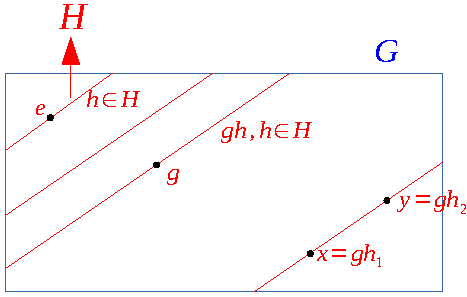
\includegraphics{images/orbits.pdf}
	\caption{Schematic representation of the set of orbits}
	\labfig{orbits}
\end{figure}
\begin{example}
Let's consider a specific rotation $g\in G=\textrm{SO}(3)$ and $h\in H=\{\textrm{rotation around the $3^{\text{rd}}$ axis}\}$. We consider all the combinations $(g\cdot h)$: the idea is that if $x$ and $y$ are in the same "orbit", $gH=\{gh: h\in H\}$, it means that $x=gh_1$ and $y=gh_2$.
\[
x^{-1}y=(gh_1)^{-1}(gh_2)=h_1^{-1}g^{-1}gh_2=h_1^{-1}h_2\in H
\]
\end{example}
We can make the idea stated in the example above more formal, by introducing the \textbf{relation H equivalence.}
\begin{definition}[Relation $\sim_H$]\index{Relation $\sim_H$}
The elements $x,y\in G$ are \textbf{H-equivalent} (hence $H\le G$) if $x^{-1}y\in H$. We write $x\sim_H y$.
\end{definition}
\begin{lemma}
$\sim_H$ is an equivalence relation in $G$.
\end{lemma}
\begin{proof}
We have to prove three properties:
\begin{enumerate}
    \item Reflective: $x\sim_H x$. 
    \[
    x^{-1}x=e\in H
    \]
    (the neutral element is in every subgroup!)
    \item Symmetry: if $x\sim_H y$ then $y\sim_H x$
    \[
    y^{-1}x=(\underbrace{x^{-1}y}_\text{{\color{red}$\in H$}})^{-1}{\color{red}\in H}
    \]
    \item Transitive: if $x\sim_H y$ and $y\sim_H z \Rightarrow x\sim_H z$
    \[
    x^{-1}z=x^{-1}(yy^{-1})z=(\underbrace{x^{-1}y}_\text{{\color{red}$\in H$}})(\underbrace{y^{-1}z}_\text{{\color{red}$\in H$}})\in H
    \]
\end{enumerate}
\end{proof}
Now we have an equivalence relation, i.e. a relation which is reflective, symmetric and transitive, then we can take the set of all the elements which are equivalent to each other: this is called an \textbf{equivalence class}.
\begin{definition}Let $H\le G$ be any subgroup. We define the \underline{\underline{\textbf{set}}} {\color{black}$G/H$} (one reads "$G$ \textbf{modulo} $H$" or "$G$ divided by $H$") as 
\[
G/H=G/\sim_H=\{\text{equivalence classes of H-equivalent elements}\}
\]
\end{definition}
By construction:\marginnote{Both the set of orbits and the set of equivalence classes are subsets of $G$.}
\[
G \underset{\mathclap{\tikz \node {$\uparrow$} node [below=1ex] {\footnotesize set of equivalence classes };}}{/} \sim_H\cong\{gH\}_{\underset{\mathclap{\tikz \node {$\uparrow$} node [below=2.5ex] {\footnotesize set of orbits };}}{g\in G}}
\]
The question now is: is the set of orbits a group itself? The answer is in general \textbf{no}. It is a group if $H$ is \textbf{normal}.
\begin{theorem}[Quotient group $G/H$]\index{Quotient group}\labthm{quotient-group}
Let $G$ be a group and {\color{red}$H\trianglelefteq G$} a \underline{\underline{\textbf{normal}}} subgroup of $G$. We define an operation between elements of $G/H$ as:
\[
g_1 H \cdot g_2 H:=(g_1g_2)H
\]
$G/H$ equipped with this product is a group.
\end{theorem}
\begin{proof}
\begin{align*}
    G/H \times G/H & \xrightarrow[]{} G/H \\
    (g_1H,g_2H) & \mapsto {\color{red}g_1g_2}H
\end{align*}
We have to check the axioms:
\begin{itemize}
    \item (G1) Associativity is left as an exercise
    \item (G2) Neutral element:
    \[
    e_{G/H}=eH=H\marginnote{The neutral element of the modulus is the coset (the "orbit") which passes through the identity.} \qquad \begin{cases}
    eH\cdot gH=egH=gH\\
    gH\cdot eH=geH=gH
    \end{cases}
    \]
    \item (G3) Inverse: $(gH)^{-1}=g^{-1}H$
\end{itemize}
\end{proof}
A question remains: when did we use the fact that the subgroup is normal? Hint: we used it implicitly in the definition of the product:
\[
\begin{cases}
g_1H & =\{g_1h:h\in H\}\\
g_2H & = \{g_2h:h\in H\}
\end{cases}\quad \Rightarrow \ g_1H \cdot g_2H=g_1h_1g_2h_2\marginnote{Here we have chosen for the first one the representative $g_1h_1$ and for the second one $g_2h_2$.}
\]
% INIZIO LEZIONE 11 07/04/2022
Short answer: In the fact that the operation $G/H$ is \textbf{indipendent of the representation}, so by using the fact that $H\trianglelefteq G$ everything is well defined.
\begin{itemize}
    \item Recall that $G/H\cong \Bqty{gH}_{g\in G}\cong G\big/ \sim_H$
    \item In $G\big/ \sim_H$, we could have that the set of equivalence classes defined by $g$ and $k$ are
    \begin{equation}\labeq{gtilde-htilde}
    \begin{split}
        \bqty{g}&=\bqty{\tilde{g}} \qquad \tilde{g}=gh_+ \quad h_+\in H\\ 
        \bqty{k}&=\bqty{\tilde{k}} \qquad \tilde{k}=kh_\ast \quad h_\ast\in H
    \end{split}
    \end{equation}
    As it is represented in \reffig{orbits2}.
\end{itemize}
\begin{figure}[h!]
	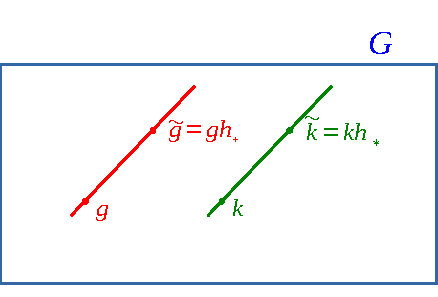
\includegraphics{images/orbits2.pdf}
	\caption{Schematic representation of the set of orbits}
	\labfig{orbits2}
\end{figure}
Now to do the product we could use either the first column or the second column, and we should get something which is the same up to h equivalence
\[
\textrm{Product: } 
\begin{cases}
\textrm{I column:} \quad \bqty{gh} &\rotatebox{-40}{$\longrightarrow$}\\
\\
\textrm{II column:} \quad \bqty{\tilde{g}\tilde{k}} &\rotatebox{40}{$\longrightarrow$}
\end{cases}
\sim_H
\]
We ask our self whether $kg\overset{?}{\sim}_H\tilde{g}\tilde{k}$, to answer we compute \marginnote{$h_\ast$ is an element of $H$ by definition}
\[
\pqty{gk}^{-1}\pqty{\tilde{g}\tilde{k}}\overset{(\ref{eq:gtilde-htilde})}{=}h^{-1}g^{-1}\pqty{gh_+kh_\ast}\overset{(G3)}{=}k^{-1}\pqty{g^{-1}g}h_+kh_\ast=\underbrace{\left({\color{red}k^{-1}}h_+ {\color{red}k}\right)}_{\text{\parbox{1.1 cm}{\centering $\in H\trianglelefteq G$ \\[-4pt]$i_{k^{-1}(h_+)}$}}}\cdot \underbrace{h_\ast}_{\in H}\in H
\]
\underline{Answer:} $gk \sim_H \tilde{g}\tilde{k}$ so the product is intrinsically defined.
\begin{kaobox}[frametitle=Remark]
We define the inner automorphism with $g^{-1}$ to the right, i.e. $i_g(h)=ghg^{-1}$, but in the computation it is on the left. It does not matter because this is the inner automorphism with respect to the element $k^{-1}$ applied to the element $h_+$, i.e. $i_{k^{-1}(h_+)}$. 
\[
\begin{split}
  i_g(h)&=ghg^{-1}\\
  i_{k^{-1}(h_+)}&=k^{-1}hk
\end{split}
\qquad \textrm{\underline{Coherent!}}
\]
The fact that $H$ is a normal subgroup is crucial in order to make this product independent from the choice of the representative.
\end{kaobox}
% 16:00
\end{document}